% -*- coding: utf-8 -*-


%%------------------------------------------------Chapter Separator-----------------------------------------------%%


\chapter{绪论}

\section{研究背景与意义}

这里来说明室内定位的研究与意义,随着物联网的快速发展,各种应用对于室内定位的需求也与日俱增,这里是测试正文中的链接的\url{https://www.baidu.com/},期望显示的不是红色。

随着无线通信、计算机和感知技术的发展,普适计算实现了物理世界和信息空间的融合,为人们提供了越来越广泛的计算和服务。普适计算中的位置感知计算变得尤为重要,因为多数服务都依赖于位置服务,而随着智能移动设备的普及,基于位置感知计算的服务也变得多种多样。目前,LBS已经成为非常有前景的研究热点之一。它能广泛支持需要动态位置信息的应用,为诸如交通导航、生活信息查询、医疗救护等提供较为准确的位置信息,因此为用户提供LBS有着巨大的市场规模和良好的商业前景。

在开阔的室外环境中,定位和导航服务主要利用全球导航卫星系统(Global Navigation Satellite System, GNSS),主要包括美国的全球定位系统(Global Positioning System, GPS)、俄罗斯的格洛纳斯系统(GLONASS)、欧洲的伽利略系统(Galileo)和中国的北斗卫星导航系统。其中,美国的GPS系统是应用最为广泛且发展较成熟的定位系统,其中民用GPS定位系统的精度可达10米左右,并且最新的GPS系统,通过地面站的位置校准等增强技术,其定位精度可以提高至2~3米左右,能够满足大多数室外LBS服务对于位置信息的精度要求。

但是,上述定位系统都不能用于室内环境下位置感知应用。由于建筑物外墙等对于卫星和基站信号的遮挡,以及复杂的室内环境带来的无线信号传播的多径效应的影响,原有技术手段和算法难以实现在室内环境下的高精度定位。与室外环境相比,室内环境更加复杂,存在着不同类型的干扰源。例如,室内建筑结构和家具等对于电磁波的传播路径的影响从而导致多径效应,来自其他无线设备的干扰和噪声等。所以,开发一种定位精度高、实时性好、经济成本低、可扩展性高的定位技术成为各大互联网企业和研究机构关注的热点课题。到目前为止,研究人员已经将多种技术和方法应用于不同场景下的室内定位系统中,其中,技术手段主要包括红外线、超声波、无线电射频识别(Radio Frequency Identification, RFID)、蓝牙、超宽带(Ultra-wide band, UWB)、地磁场以及无线局域网(802.11, Wi-Fi)等。



\section{室内定位技术分类}

这里想通过室内定位技术的分类来引出指纹定位和行人航位推算技术的详细介绍。

典型的Wi-Fi位置指纹定位算法大体上可以分为两类,即基于近邻选择和基于机器学习的算法。基于近邻选择的算法主要有NN、kNN和w-kNN。近邻选择算法将在线采集到的RSS作为特征值,将其和离线阶段获得的指纹数据库中的RSS样本进行匹配并选择其中最相似的一个或者k个参考点,通过平均或者加权平均k个参考点的位置坐标作为定位结果。基于机器学习的位置指纹定位算法利用离线采集的RSS样本训练确定性或者概率性数学模型,进行确定模型参数,得到一个RSS样本作为输入、位置坐标作为输出的映射关系。在在线阶段,将在线RSS作为模型输入,计算得出定位结果。基于机器学习的位置指纹定位算法有ANN和SVR等。由于RSS的动态变化,典型的Wi-Fi位置指纹定位算法存在着定位结果稳定性比较差的问题。如图XX所示,在同一位置来自同一个无线热点(AP)的RSS的变化情况。

\subsection{行人航位推算}
这里详细说明行人航位推算的原理,以及简单的说明行人航位推算技术的优缺点




\section{结构化空间和开放空间的定义}

这一小节的位置还有待后续斟酌,当前先放在这里吧。

这里给出关于结构化空间和开放空间的抽象定义,用于后续讨论的基础,这里最好给出一个相对详细且抽象的定义,因为这两个概念的定义是后续讨论的基础,所以这里的定义最好能够给人以信服,且最好能够通过引用权威论文来加强说服力,在这一方面,当前还是存在着一定的困难。

\section{国内外研究现状}

国内外研究现状需要从室内定位中与本文相关的部分来进行总结,并且需要设计到较多的参考文献,并且这里的行文的说法也很重要,国内外研究现状的篇幅大概在2-3页。

\section{本文的主要工作以及章节安排}

本文的主要工作应该包括全文的一个整理思路,后续章节中隐含的逻辑关系也应该从这里得到清晰的了解,并且最好通过一个简单清晰的图来说明。


%%------------------------------------------------Chapter Separator-----------------------------------------------%%


\chapter{行人定位算法概述}

\section{典型的Wi-Fi定位算法}

这里介绍典型的Wi-Fi定位算法,例如kNN、Bayes和SVR等。

\section{行人航位推算原理}

这里介绍行人航位推算的原理,行人航位推算的原理图可以放到这里来。

\begin{figure}[htb]
	\centering
	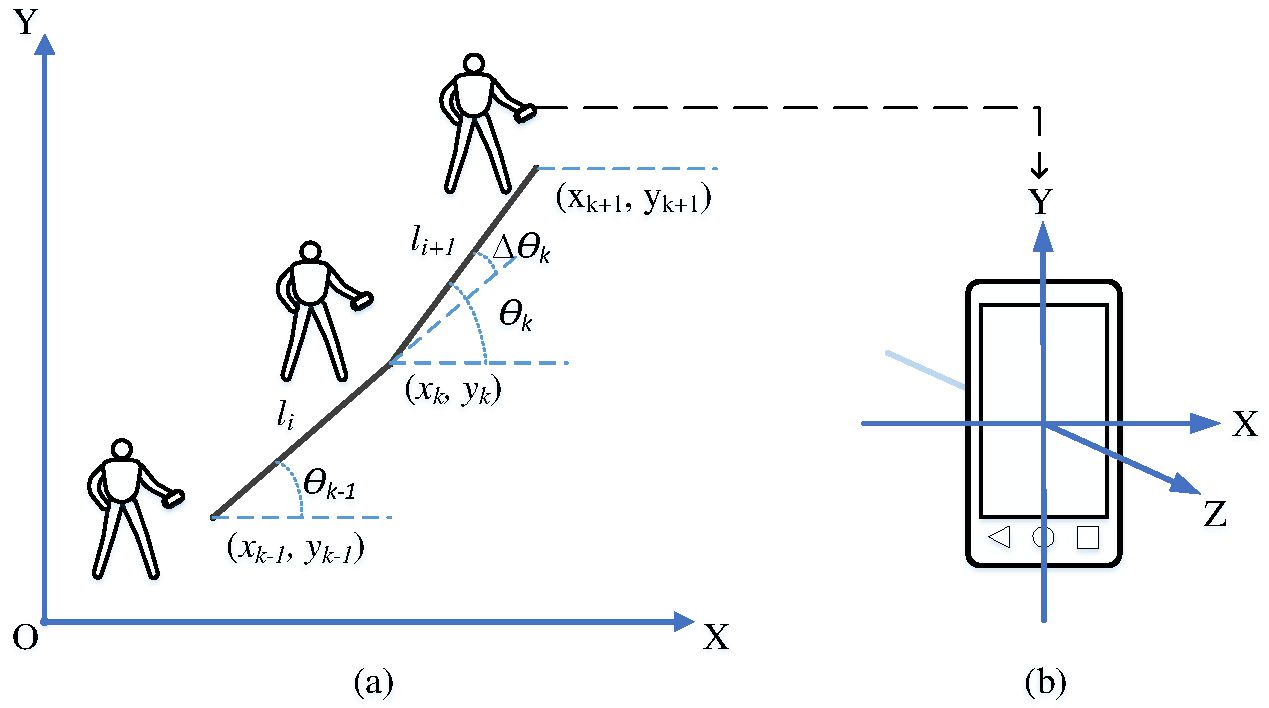
\includegraphics[width=4.75in]{./figures/2/IndoorPos-PDRSchema}
	\caption{行人航位推算原理示意图 (a)全局坐标系下行人航位推算;(b)设备坐标系。}
	\label{fig-pdr}
\end{figure}

\section{主要的滤波算法}

这里介绍卡尔曼滤波和粒子滤波的算法的数学模型和适用情况。

\section{实验环境}

这里主要描述用于后续文章实验的实验场景,其中主要包括实验环境,智能移动设备和参试人员的介绍等。

\section{本章小结}

在这里主要是总结这一章节的内容,如果必要,可以特别简单的引出下一章节的内容。


%%------------------------------------------------Chapter Separator-----------------------------------------------%%


\chapter{面向大规模结构化空间中的行人自主定位}

\section{引言}

在引言中必须说明该章节想要解决的主要问题,并且对问题进行一个简要清晰的描述,一便于后续的理解。

室内定位技术多种多样,但是在实际应用中还存在着许多问题,本章主要从成本和安全两个方面来考量。

\section{模型建立}

模型建立小节主要来详细说明算法的设计细节。

\section{实验分析}

通过实验来对算法中的参数或者目标进行对比分析。

\section{本章小节}

针对引言中所给出的问题,总结本章。


%%------------------------------------------------Chapter Separator-----------------------------------------------%%


\chapter{从结构化空间到开发空间:基于众源的行人定位}

\section{引言}

在引言中必须说明该章节想要解决的主要问题,并且对问题进行一个简要清晰的描述,一便于后续的理解。

考虑到公共空间,如商场、体育馆、火车站、地铁站等,其室内建筑结构不仅包含结构化空间,还包含开发空间,而从结构化空间进入开放空间以后,由于缺少地标点,进而基于PDR技术的行人定位的实现存在着较大的困难,本章中讨论通过基于众源的AP热点位置估计算法来实现行人从结构化空间到开放空间的无缝定位。

\section{模型建立}

模型建立小节主要来详细说明算法的设计细节。

\section{实验分析}

通过实验来对算法中的参数或者目标进行对比分析。

\section{本章小节}

针对引言中所给出的问题,总结本章。


%%------------------------------------------------Chapter Separator-----------------------------------------------%%


\chapter{基于众源生成的Wi-Fi指纹库的定位技术研究与分析}

\section{引言}

在引言中必须说明该章节想要解决的主要问题,并且对问题进行一个简要清晰的描述,一便于后续的理解\cite{montoliu2017indoorloc}。

基于众源生成的Wi-Fi指纹库由于指纹生成方式的不同,相比于通过专业人士现场测量而得到的Wi-Fi指纹库,存在着两个主要的不同点,一个是由于上传指纹位置的随机性而导致的指纹数据覆盖范围的不平衡性;一个是由于上传指纹的设备的多样性而导致的指纹数据的不一致性。

\section{模型建立}

模型建立小节主要来详细说明算法的设计细节。

\subsection{精度自定义}



\section{实验分析}

通过实验来对算法中的参数或者目标进行对比分析。

\section{本章小节}

针对引言中所给出的问题,总结本章。


%%------------------------------------------------Chapter Separator-----------------------------------------------%%


\chapter{定位技术在Android平台上的实现}

\section{Android平台简介}

在智能手机领域,Android操作系统自从上市以来,凭借其良好的运行性能和方便的开发环境迅速占领了智能手机市场,如表\ref{tab-61}所示,根据市场调研机构Gartner在2018年2月份发布了一份报告显示2017年全年Android手机市占率高达85.9\%\cite{gartner-smartphone-2017}。


\begin{table} [thb]
	\caption{2017年全球智能手机销售给最终用户统计}\label{tab-61}
	\small
	\centering
	%[t]
	{
		\begin{tabular}{c c c c c}
			\toprule
			操作系统 & 2017(千部) & 2017市场占有率(\%) & 2016(千部) & 2016市场占有率(\%)\\
			\midrule
			Android & 1320118.1 & 85.9 & 1268562.7 & 84.8\\
			iOS & 214924.4 & 14.0 & 216064.0 & 14.4\\
			其他 & 1493.0 & 0.1 & 11332.2 & 0.8\\
			总计 & 1536535.5 & 100.0 & 1495959.0 & 100.0\\			
			\bottomrule
		\end{tabular}
	}
\end{table}


\section{定位技术实现}

在本小节中给出基于Android平台实现过程中遇到的问题,比如设计到众源算法时需要提高算法的处理时间等。

\section{公开数据集的建立}

通过多个Android手机平台上运行定位APP,进而建立公开的数据集方便后续其他定位技术的研究人员来进行定位算法的对比实验研究。


%%------------------------------------------------Chapter Separator-----------------------------------------------%%


\chapter{总结与展望}

\section{本文总结}

现在的定位算法没有考虑手机不同的携带位置对于定位结果的影响。

随着物联网技术的发展和智能移动设备的普及,特别是未来可穿戴设备如智能手环、智能手表、智能眼镜的流行,基于位置的服务在日常出行、医疗监护、应急救援、智能广告等各种方面展示了良好体验和应用前景,因此越来越受到人们的关注和重视。近年来,由于WLAN已经广泛布置于室内环境,基于Wi-Fi的位置指纹定位技术倍受人们的青睐并成为当前国内外的研究热点。本文在对Wi-Fi位置指纹定位各个关键环节深入研究的基础上,以通过众源的方式提高位置指纹数据库的构建效率、定位算法的可扩展性。

\section{后续工作安排}

总结本文,并给出后续的工作安排。

本文的定位技术主要面向室内二维平面的定位,虽然在引入楼层的信息后,上述定位技术很容易扩展至整栋建筑的室内定位,但是上述定位技术并不能给出定位目标的高度信息。

本文给出的定位技术的定位精度都在1~3米级别,面对物联网应用中对于室内高精度的定位需求,本文讨论的算法在定位精度上还不能满足

在现有研究基础上,未来将继续对组合定位算法进行优化,以提高算法的定位精度、可扩展性和可靠性。同时,未来将针对更多的运动模式和导航场景进行研究,以提高算法适用性,将定位算法扩展到更多应用领域,如智能手表、智能眼镜等可穿戴设备上。更进一步挖掘用户导航数据,提高众源数据库的质量和效率。具体可以从以下几个方面进行研究:

\begin{enumerate}[1{)}]
	\item 考虑将基于遗传算法的路径规划算法运用在地磁匹配算法中进一步提高指纹匹配算法的使用效率;
	\item 结合地图匹配技术,利用地图信息进一步提高定位可靠性和定位精度。
	\item 目前组合定位算法针对的行人日常行走的模式,未来针对人在汽车、骑车、跑步等更多运动模式进行进一步的研究,扩展算法的应用领域;
	\item 室内外低能耗的无缝定位是未来的发展趋势,因此定位系统需要考虑将室内和室外定位信息融合,以实现无处不在的定位服务;
	\item 个人隐私和保护越来越受到人们的重视,因此未来的定位系统特别需要考虑在定位过程中对于被服务者的个人隐私的保护的研究。
\end{enumerate}

%%------------------------------------------------Chapter Separator-----------------------------------------------%%


\chapter{南开大学学位论文格式宏包 NKThesis 使用说明} \label{chpt:A}

\section{系统要求}

模板仅在 TeXLive 2016 下测试通过。对于其它 TeX 发行版可能需要做个别修改。


\section{NKThesis 使用说明}

本模板可以使用以下两种方式编译:
\begin{enumerate}
 \item PDF\LaTeX

 \item \XeLaTeX [推荐]
\end{enumerate}

例如,
\begin{verbatim}
         pdflatex main
         bibtex main     % 处理参考文献
         pdflatex main   % 连续编译两遍
         pdflatex main   % 以生成正确的文献引用。
\end{verbatim}

本模板用到 宋体、楷体、仿宋、黑体四种字体\cite{GB25100—2010}. 若需重新配置字体, 请修改 NKTfonts.cfg.
对于 Linux/Mac 下的 TeX Live 2009, 可能需要设置环境变量 OSFONTDIR, 具体内容请参考 texmf.cnf.

我们建议您使用\XeLaTeX\ 编译。与前两种方法相比,\XeLaTeX\  编译长文档的速度更快,
编译一篇一百多页的论文只需几秒的时间(SL9400 @ 1.86GHz)。

在改变编译方式前应先删除 *.toc 和 *.aux 文件,
因为不同编译方式产生的辅助文件格式可能并不相同。

注意:使用 \XeLaTeX\ 编译时,\XeTeX\ 的版本应不低于 0.9995.0(MiKTeX 2.8 或者 TeXLive 2009)。


\section{引用章节号}
\label{sec:ex:A}

引用章节号请参考如下格式: \ref{chpt:A}\ref{sec:ex:A}.


\section{中英文间隔}

使用 \XeLaTeX\ 编译时,会自动在中英文转换时添加必要的空格。 使用 [PDF]\LaTeX\
编译时仅忽略中文之间的空格,而中英文之间的空格予以保留。
因此,不管何种编译方式,您都不需要在中英文间添加 $\tilde{}$ 以获得额外的空格。例如,

这是 English 中文 $x=y$ 测试

这是English中文$x=y$测试

可以看出,以上两行用 \XeLaTeX\ 编译的结果是相同的。


%%------------------------------------------------Chapter Separator-----------------------------------------------%%


\chapter{引言}

\section{研究背景}

随着计算机技术和互联网技术的快速发展\cite{Nadkarni-1992},各式各样的网络应用伴随着人们的需求应运而生\cite{Hua-Wang-1973}。

\subsection{研究意义}

随着计算机技术和互联网技术的快速发展\cite{Nadkarni-1992},各式各样的网络应用伴随着人们的需求应运而生\cite{Hua-Wang-1973}。

\begin{table} [thb]
	\caption{常见端口协议映射表}\label{tab:21}
	\small
	\centering
	%[t]
	{
		\begin{tabular}{cccc}
			\toprule
			Port & Protocol & Port & Protocol\\
			\midrule
			21 & FTP & 88 & Kerberos\\
			22 & SSH & 109 & POP\\
			23 & Telnet & 110 & POP3\\
			25 & SMTP & 115 & SFTP\\
			37 & TIME & 143 & IMAP4\\
			43 & WHOIS & 161 & SNMP\\
			53 & DNS & 179 & BGP\\
			80 & HTTP & 443 & HTTPS\\
			
			\bottomrule
		\end{tabular}
	}
\end{table}

网络流量的不断增长给网络管理带来了巨大难题。

\begin{figure}[htb]
\centering

\includegraphics[width=3.8in]{./figures/0/nankaidaxue}
\caption{南开大学标准图片}
\label{fig:11}
\end{figure}

近几年来,随着手机、平板电脑、智能手环等移动设备的普及\supercite{bahl2000radar},移动互联网用户不断增多\supercite{monkey}。